\subsection{Реализация прошивки}
Необходимо учитывать тот факт, что флеш-память ограничена 2 МБ. Часть этого пространства должна быть зарезервирована для прошивки, часть для веб-приложения и часть для пользовательских данных. Веб-приложение должно быть как можно меньше, чтобы поместиться во флеш-память вместе с изображениями, шрифтами, библиотеками и другими необходимыми данными. 

\subsubsection{SDK от Realtek}
SDK реализован на языке C в соответствии со стандартом gnuc99.

Для создания прошивки использовался официальный SDK для платформы Ameba-One от компании Realtek.
Использовался SDK версии 4.0b.
В процессе разработки в SDK были внесены существенные изменения. Был выброшен функционал необходимый для только при сборке для платформы Ameba-Zero. Был создан порт более новой версии LwIP 1.5 взамен присутствующему в SDK 1.4. Была проведена замена GNU GCC ARM Toolchain с версии 4.8 на версию 8.1. Также FreeRTOS была обновлена с версии 6.2 до версии 8.1.4. Были исправлены многочисленные предупреждения компилятора при компиляции SDK. В частности были разрешены свыше 80 предупреждений о неявном определении функции (implicit-function-declaration). Данного диагностическое сообщение компилятора явлается предупреждением из-за исторических причин, однако его наличие в современном проекте и особенно в SDK явно указывает что к данному следует относится как к ошибке. Также из SDK был выкинут функционал отвечающий за работу с форматом XML, протоколом WPS, брокером MQTT, и другими модулями системы которые не использовались в данной работе. Некоторые специализированные настройки для LwIP и FreeRTOS приходилось производить в исходных файлах SDK, так как не было возможности включить или выключить функционал из файлов пользовательского проекта или в файле сборки.


\subsubsection{GNU GCC ARM Toolchain}
При работе с SDK было принято решение произвести обновление версии GNU GCC ARM Tollchain с версии 4.8, которая поставлялась вместе с SDK, на версию 8.1, которая была доступна на официальном сайте ARM.
К сожалению данная замена не дала серьезной оптимизации в плане размера бинарного файла, улучшение составили примерно 5\%. Уменьшение размера бинарного файла, позволяет освободить память RAM микроконтроллера и осбободить флеш-память микроконтроллера для хранения веб-приложения и пользовательских настроек.

\subsubsection{Среда разработки}
Вся разработка прошивки велась на операционной системе Linux. Для редактирования исходных кодов использовался редактор VIM с плагином YouCompleteMe. Также использовались и другие стандартные утилиты системы Linux. Для поиска и навигации по проекту и SDK использовалась программа TheSilverSearcher. Для прошивки программы в микроконтроллер использовалась программа OpenOCD в тандеме с GDB (Gnu Debugger). Для контроля версий использовалась программа Git.


\subsubsection{Инструменты разработки и отладки от ARM}
Компания ARM предоставляет набор инструментов для разработчиков. В данной работе использовались такие разработки как прошивка DAPLink, а также алтернатива OpenOCD под названием pyOCD.
Рисунок ниже описывает способ подключения к микроконтроллеру от компьютера. Прошивка DAPLink предназначенна для установки на устройстве помеченном как Programmer/debug probe.

\begin{figure}[h!]
    \centering
    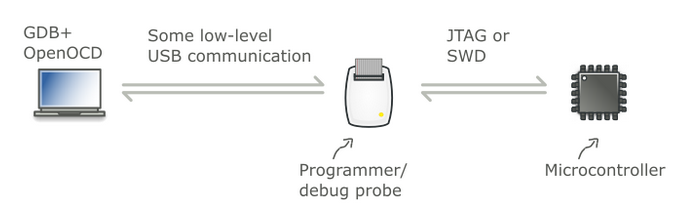
\includegraphics[width=0.9\textwidth]{pc_to_mcu.png}
    \caption{Способ подключения к микроконтроллеру от компьютера.}
\end{figure}


\subsubsection{Инструменты создания образа файловой системы}
В данной работе для создания и организации файловой системы во флеш-памяти микроконтроллера использовался проект SPIFFS.  Для создания образа файловой системы использовался проект mkspiffs, который реализует функции SPIFFS используя стандартную библиотеку С. Проект mkspiffs таким образом позволяет создать образ файловой системы из файлов в директории. После чего данных образ загружается во флеш-память модуля по определенному адресу.


\subsubsection{Цикл разработки}
Одна итерация разработки выглядела следующим образом. Сначала вносились изменения в файлы проекта, неважно пользовательской прошивки или официального SDK. После этого запускалась компиляция программы. При условии успешной компиляции, происходил запуск скрипта-настройщика для OpenOCD. После старта OpenOCD процессса, запускался скрипт-настройщик для GDB. Данный скрипт командовал GDB подключиться к процессу OpenOCD и инициировать загрузку .bin файла во флеш память. Данная процедура была необходима, поскольку программа OpenOCD предоставляет канал между GDB и микроконторллером, а GDB известно какие команды применимы для ядра ARM Cortex-M3 чтобы загрузить бинарный файл во флеш-память. 

\subsubsection{Использование языка Rust}
В данной работе исследовалась возможность программирования микроконторллера на языке Rust, в качестве более безопасной альтернативы языку C.

Безопасность и надежность всегда являются первостепенными задачами. Если прошивка была бы написана на языке программирования Rust, это ограничило бы количество ошибок связанных с переполнением буфера, стека и ряда других типичных для приложений написанных на языке C. Использование Rust также должно было бы упростить тестирование, поскольку юнит-тесты являются частью языка, что будет способствовать поддержанию качество кода. Использование Wi-Fi модуля на основе ARM означает, что Rust может использоваться в качестве языка программирования.

К сожалению задача компиляции языка Rust для данной платформы, а также его интеграция с SDK и уже созданными модулями написаными на С, оказались не тривиальны. Во-первых, для компиляции требовалось подключить LLVM ARM Toolchain, во-вторых многие функции на языке С переопределяются макросами препроцессора, в частности это касается стандартной библиотеки и проекта FreeRTOS, для которых приходится создавать оберточные функции. Это требует больших трудозатрат. После долгих экспериментов пришлось отказаться от использования языка Rust в данной работе.



\subsection{Реализация одно-страничного веб-приложения}
Необходимо учитывать тот факт, что флеш-память ограничена 2 МБ.

\subsubsection{Набор инструментов разработки}
Для разработки использовался текстовый редактор VIM. Система контроля версий Git. Используемые технологии Javascript, CSS, HTML.

\subsubsection{Используемые библиотеки}
Вначале разработки использовалась библиотека Twitter Bootstrap, однако впоследствии от нее пришлось отказаться из-за ее большого размера и вести разработку на более низком уровне.
Также на первых этапах разработки для показа диалогового окна использовалась библиотека tingle, которая впоследствии была заменена на внутренную библиотеку.

\subsubsection{Система сборки}
Задажей системы сборки является из проверить входные файлы на корректность (lint), скомпановать исходники, ужать картинки, оптимизировать шрифты и заархивировав поместить в каталог /dist готовые файлы для веб-приложения.

Для сборки используется система Gulp. В процессе сборки задействовано огромное количество nodejs плагинов. 
Система сборки является одной из самых сложных и многоуровневых частей веб-приложения. 

На первом этапе HTML проходит строгую проверку на корректность и на качество кода. Проверяются от ошибки в опечатках названий элементов до стиля написания id аттрибутов (всегда низкие буквы через нижнее подчеркивание). Для проверки используется пакет htmlhint. 
Ниже представленна конфигурация для запуска htmlmin.

\begin{small}
\begin{verbatim}
    var htmlhintconfig = {
        "tagname-lowercase": true,
        "attr-lowercase": true,
        "attr-value-double-quotes": true,
        "attr-value-not-empty": false,
        "attr-no-duplication": true,
        "doctype-first": true,
        "tag-pair": true,
        "tag-self-close": false,
        "spec-char-escape": true,
        "id-unique": true,
        "src-not-empty": true,
        "title-require": true,
        "alt-require": true,
        "doctype-html5": true,
        "id-class-value": "underscore",
        "style-disabled": false,
        "inline-style-disabled": false,
        "inline-script-disabled": false,
        "space-tab-mixed-disabled": "space",
        "id-class-ad-disabled": false,
        "href-abs-or-rel": false,
        "attr-unsafe-chars": true,
        "head-script-disabled": true
    };
\end{verbatim}
\end{small}


После этого в элемент <head> вставляются два аттрибута с текущей датой-временем и хеш значением последнего коммита в системе Git. Далее в файле заменяются ссылки на файлы .css и .js так как в процессе сборки некоторые файлы будут объеденены в один модуль. Следующим шагом является копирование преобразованного HTML в каталог /debug. Последний шаг это оптимизация HTML удаляющая комментарии с пробелы где это возможно и копирование файла в каталог /dist. 

Следующий шаг - создание единой картинки-спрайта из нескольких картинок которые необходимы в веб-интерфейсе. На данном этапе все картинки PNG объединяются в одну. Оптимизации еще не применяются.
На выходе в каталоге появляется единая картинка spritesheet-bundle.png и .css файл описывающий положение и размер каждой из картинок на единой картинке-спрайте.

После создания единой картинки-спрайта идет верификация и сборка файлов CSS.  

Для верификации CSS используется программа PostCSS и набор плагинов к ней. В частности используется плагин Browserlist для задания списка поддерживаемых браузеров. Список браузеров необходим для плагина Autoprefix который автоматически добавляет префиксы к определенным дескрипторам CSS, если дескрипторы без префикса не поддерживаются в заявленных браузерах.

Далее модули разделяются на те которые были импортированы в проект, например reset.css который разрабатываетяс сообществом, и те модули которые были разработаны для проекта. Инпортированные модули не проходят дополнительные проверки, кроме Autoprefix. После этого они минифицируются с помощю программы clean-css и цопируются в каталоги /debug и /dist.
Модули css которые были созданны в рамках данного проекта подвергаются дополнительной обработке. Во-первых, в модулях используются специальные директивы, которые не входят в стандарт CSS, данные директивы обрабатываются PostCSS плагинам simplevars, который позволяет объявлять переменные в css модулях, и nestedcss, который позволяет писать более простые для понимания вложенные css стили. Данные плагины позволяют расширить синтаксис CSS для упрощения разработки и поддержки кода. После работы данных двух плагинов, запускается еще один PostCSS плагин - stylelint, который проверяет css на корректность и качество кода. Ниже приведена конфигурация плагина stylelint.

\begin{small}
\begin{verbatim}
    var lintconfig = {
        ignoreFiles: [
            // ignore sprites css file generated by spritesmith tool
            'spritesheet.css',
        ],
        rules: {
            // the stylelint-config-recommended, it turns on all the possible errors rules within stylelint
            "at-rule-no-unknown": true,
            "block-no-empty": true,
            "color-no-invalid-hex": true,
            "comment-no-empty": true,
            "declaration-block-no-duplicate-properties": [
                true,
                {
                    ignore: ["consecutive-duplicates-with-different-values"]
                }
            ],
            "declaration-block-no-shorthand-property-overrides": true,
            "font-family-no-duplicate-names": true,
            "font-family-no-missing-generic-family-keyword": true,
            "function-calc-no-unspaced-operator": true,
            "function-linear-gradient-no-nonstandard-direction": true,
            "keyframe-declaration-no-important": true,
            "media-feature-name-no-unknown": true,
            "no-descending-specificity": true,
            "no-duplicate-at-import-rules": true,
            "no-duplicate-selectors": true,
            "no-empty-source": true,
            "no-extra-semicolons": true,
            "no-invalid-double-slash-comments": true,
            "property-no-unknown": true,
            "selector-pseudo-class-no-unknown": true,
            "selector-pseudo-element-no-unknown": true,
            "selector-type-no-unknown": true,
            "string-no-newline": true,
            "unit-no-unknown": true,
            // the stylelist-config-standart, turns on additional rules to enforce common stylistic conventions
            "at-rule-empty-line-before": [ "always", {
                except: [
                    "blockless-after-same-name-blockless",
                    "first-nested",
                ],
                ignore: ["after-comment"],
            } ],
            "at-rule-name-case": "lower",
            "at-rule-name-space-after": "always-single-line",
            "at-rule-semicolon-newline-after": "always",
            "block-closing-brace-empty-line-before": "never",
            "block-closing-brace-newline-after": "always",
            "block-closing-brace-newline-before": "always-multi-line",
            "block-closing-brace-space-before": "always-single-line",
            "block-opening-brace-newline-after": "always-multi-line",
            "block-opening-brace-space-after": "always-single-line",
            "block-opening-brace-space-before": "always",
            "color-hex-case": "lower",
            "color-hex-length": "short",
            "comment-empty-line-before": [ "always", {
                except: ["first-nested"],
                ignore: ["stylelint-commands"],
            } ],
            "comment-whitespace-inside": "always",
            "custom-property-empty-line-before": [ "always", {
                except: [
                    "after-custom-property",
                    "first-nested",
                ],
                ignore: [
                    "after-comment",
                    "inside-single-line-block",
                ],
            } ],
            "declaration-bang-space-after": "never",
            "declaration-bang-space-before": "always",
            "declaration-block-semicolon-newline-after": "always-multi-line",
            "declaration-block-semicolon-space-after": "always-single-line",
            "declaration-block-semicolon-space-before": "never",
            "declaration-block-single-line-max-declarations": 1,
            "declaration-block-trailing-semicolon": "always",
            "declaration-colon-newline-after": "always-multi-line",
            "declaration-colon-space-after": "always-single-line",
            "declaration-colon-space-before": "never",
            "declaration-empty-line-before": [ "always", {
                except: [
                    "after-declaration",
                    "first-nested",
                ],
                ignore: [
                    "after-comment",
                    "inside-single-line-block",
                ],
            } ],
            "function-comma-newline-after": "always-multi-line",
            "function-comma-space-after": "always-single-line",
            "function-comma-space-before": "never",
            "function-max-empty-lines": 0,
            "function-name-case": "lower",
            "function-parentheses-newline-inside": "always-multi-line",
            "function-parentheses-space-inside": "never-single-line",
            "function-whitespace-after": "always",
            "indentation": 4,
            "length-zero-no-unit": true,
            "max-empty-lines": 1,
            "media-feature-colon-space-after": "always",
            "media-feature-colon-space-before": "never",
            "media-feature-name-case": "lower",
            "media-feature-parentheses-space-inside": "never",
            "media-feature-range-operator-space-after": "always",
            "media-feature-range-operator-space-before": "always",
            "media-query-list-comma-newline-after": "always-multi-line",
            "media-query-list-comma-space-after": "always-single-line",
            "media-query-list-comma-space-before": "never",
            "no-eol-whitespace": true,
            "no-missing-end-of-source-newline": true,
            "number-leading-zero": "always",
            "number-no-trailing-zeros": true,
            "property-case": "lower",
            "rule-empty-line-before": [ "always-multi-line", {
                except: ["first-nested"],
                ignore: ["after-comment"],
            } ],
            "selector-attribute-brackets-space-inside": "never",
            "selector-attribute-operator-space-after": "never",
            "selector-attribute-operator-space-before": "never",
            "selector-combinator-space-after": "always",
            "selector-combinator-space-before": "always",
            "selector-descendant-combinator-no-non-space": true,
            "selector-list-comma-newline-after": "always",
            "selector-list-comma-space-before": "never",
            "selector-max-empty-lines": 0,
            "selector-pseudo-class-case": "lower",
            "selector-pseudo-class-parentheses-space-inside": "never",
            "selector-pseudo-element-case": "lower",
            "selector-pseudo-element-colon-notation": "double",
            "selector-type-case": "lower",
            "unit-case": "lower",
            "value-list-comma-newline-after": "always-multi-line",
            "value-list-comma-space-after": "always-single-line",
            "value-list-comma-space-before": "never",
            "value-list-max-empty-lines": 0,
            // our rules, place below
            "property-no-vendor-prefix": true,
            "selector-no-vendor-prefix": true,
            "at-rule-no-vendor-prefix": true,
            "value-no-vendor-prefix": true,
            "declaration-no-important": true,
        }
    };
\end{verbatim}
\end{small}

 Далее css модули проверяются на наличие директив которые появились в последних версиях стандарта CSS и которые не обрабатываются на более старых версиях браузеров. Данная проверка осуществляетяс с помощю PostCSS плагина doiuse, который опирается на базу данных проектов Caniuse и Browserlist. 
 
 
Модули которые были разработаны в рамках данного проекта также обрабатываются плагином Autoprefix. Наконец css копируется в каталог /debug и его минифицированная версия копируются в каталог /dist. Ниже приведены насторйки для данной проверки. Браузер OperaMini исключен из списка, поскольку информация о нем, которая имеется в проектах Caniuse и Browserlist не соответствует действительности. Это вызывает большое количество ложных предупреждений.  

\begin{small}
\begin{verbatim}
var ourbrowsers = ['> 0.05% in RU', 'not ie < 10', 'not OperaMini all'];
\end{verbatim}
\end{small}


После сборки CSS модулей, производится сборка Javascript модулей. Так же как и в случае сборки CSS модулей, несколько Javascript файлов могут объединятся в один модуль. После этого для модулей которые взяты из сообщества, как наприер fullcalendar.js, без дополнительных проверок создаются две копии, вторая из которых минимизируется и файлы копируются в каталоги /debug и /dist для неминифицированной и минифицированной версии соответственно. Модули были написаны в рамках данной работы, подвергаются дополнительной проверке с помосщю программы eslint. Ниже приведена конфигурация для eslint.  

\begin{small}
\begin{verbatim}
    var eslintconf = {
        rules: {
            "accessor-pairs": "off",
            "array-bracket-newline": "off",
            "array-bracket-spacing": "off",
            "array-callback-return": "off",
            "array-element-newline": "off",
            "arrow-body-style": "off",
            "arrow-parens": "off",
            "arrow-spacing": "off",
            "block-scoped-var": "off",
            "block-spacing": "off",
            "brace-style": "off",
            "callback-return": "off",
            "camelcase": "off",
            "capitalized-comments": "off",
            "class-methods-use-this": "off",
            "comma-dangle": "off",
            "comma-spacing": "off",
            "comma-style": "off",
            complexity: "off",
            "computed-property-spacing": "off",
            "consistent-return": "off",
            "consistent-this": "off",
            "constructor-super": "warn",
            curly: "off",
            "default-case": "off",
            "dot-location": "off",
            "dot-notation": "off",
            "eol-last": "off",
            eqeqeq: "off",
            "func-call-spacing": "off",
            "func-name-matching": "off",
            "func-names": "off",
            "func-style": "off",
            "function-paren-newline": "off",
            "generator-star-spacing": "off",
            "getter-return": "off",
            "global-require": "off",
            "guard-for-in": "off",
            "handle-callback-err": "off",
            "id-blacklist": "off",
            "id-length": "off",
            "id-match": "off",
            "implicit-arrow-linebreak": "off",
            indent: "off",
            "indent-legacy": "off",
            "init-declarations": "off",
            "jsx-quotes": "off",
            "key-spacing": "off",
            "keyword-spacing": "off",
            "line-comment-position": "off",
            "linebreak-style": "off",
            "lines-around-comment": "off",
            "lines-around-directive": "off",
            "lines-between-class-members": "off",
            "max-depth": "off",
            "max-len": "off",
            "max-lines": "off",
            "max-nested-callbacks": "off",
            "max-params": "off",
            "max-statements": "off",
            "max-statements-per-line": "off",
            "multiline-comment-style": "off",
            "multiline-ternary": "off",
            "new-cap": "off",
            "new-parens": "off",
            "newline-after-var": "off",
            "newline-before-return": "off",
            "newline-per-chained-call": "off",
            "no-alert": "off",
            "no-array-constructor": "off",
            "no-await-in-loop": "off",
            "no-bitwise": "off",
            "no-buffer-constructor": "off",
            "no-caller": "off",
            "no-case-declarations": "warn",
            "no-catch-shadow": "off",
            "no-class-assign": "warn",
            "no-compare-neg-zero": "warn",
            "no-cond-assign": "warn",
            "no-confusing-arrow": "off",
            "no-console": "warn",
            "no-const-assign": "warn",
            "no-constant-condition": "warn",
            "no-continue": "off",
            "no-control-regex": "warn",
            "no-debugger": "warn",
            "no-delete-var": "warn",
            "no-div-regex": "off",
            "no-dupe-args": "warn",
            "no-dupe-class-members": "warn",
            "no-dupe-keys": "warn",
            "no-duplicate-case": "warn",
            "no-duplicate-imports": "off",
            "no-else-return": "off",
            "no-empty": "warn",
            "no-empty-character-class": "warn",
            "no-empty-function": "off",
            "no-empty-pattern": "warn",
            "no-eq-null": "off",
            "no-eval": "off",
            "no-ex-assign": "warn",
            "no-extend-native": "off",
            "no-extra-bind": "off",
            "no-extra-boolean-cast": "warn",
            "no-extra-label": "off",
            "no-extra-parens": "off",
            "no-extra-semi": "warn",
            "no-fallthrough": "warn",
            "no-floating-decimal": "off",
            "no-func-assign": "warn",
            "no-global-assign": "warn",
            "no-implicit-coercion": "off",
            "no-implicit-globals": "off",
            "no-implied-eval": "off",
            "no-inline-comments": "off",
            "no-inner-declarations": "warn",
            "no-invalid-regexp": "warn",
            "no-invalid-this": "off",
            "no-irregular-whitespace": "warn",
            "no-iterator": "off",
            "no-label-var": "off",
            "no-labels": "off",
            "no-lone-blocks": "off",
            "no-lonely-if": "off",
            "no-loop-func": "off",
            "no-magic-numbers": "off",
            "no-mixed-operators": "off",
            "no-mixed-requires": "off",
            "no-mixed-spaces-and-tabs": "warn",
            "no-multi-assign": "off",
            "no-multi-spaces": "off",
            "no-multi-str": "off",
            "no-multiple-empty-lines": "off",
            "no-native-reassign": "off",
            "no-negated-condition": "off",
            "no-negated-in-lhs": "off",
            "no-nested-ternary": "off",
            "no-new": "off",
            "no-new-func": "off",
            "no-new-object": "off",
            "no-new-require": "off",
            "no-new-symbol": "warn",
            "no-new-wrappers": "off",
            "no-obj-calls": "warn",
            "no-octal": "warn",
            "no-octal-escape": "off",
            "no-param-reassign": "off",
            "no-path-concat": "off",
            "no-plusplus": "off",
            "no-process-env": "off",
            "no-process-exit": "off",
            "no-proto": "off",
            "no-prototype-builtins": "off",
            "no-redeclare": "warn",
            "no-regex-spaces": "warn",
            "no-restricted-globals": "off",
            "no-restricted-imports": "off",
            "no-restricted-modules": "off",
            "no-restricted-properties": "off",
            "no-restricted-syntax": "off",
            "no-return-assign": "off",
            "no-return-await": "off",
            "no-script-url": "off",
            "no-self-assign": "warn",
            "no-self-compare": "off",
            "no-sequences": "off",
            "no-shadow": "off",
            "no-shadow-restricted-names": "off",
            "no-spaced-func": "off",
            "no-sparse-arrays": "warn",
            "no-sync": "off",
            "no-tabs": "off",
            "no-template-curly-in-string": "off",
            "no-ternary": "off",
            "no-this-before-super": "warn",
            "no-throw-literal": "off",
            "no-trailing-spaces": "off",
            "no-undef": "warn",
            "no-undef-init": "off",
            "no-undefined": "off",
            "no-underscore-dangle": "off",
            "no-unexpected-multiline": "warn",
            "no-unmodified-loop-condition": "off",
            "no-unneeded-ternary": "off",
            "no-unreachable": "warn",
            "no-unsafe-finally": "warn",
            "no-unsafe-negation": "warn",
            "no-unused-expressions": "off",
            "no-unused-labels": "warn",
            "no-unused-vars": "warn",
            "no-use-before-define": "off",
            "no-useless-call": "off",
            "no-useless-computed-key": "off",
            "no-useless-concat": "off",
            "no-useless-constructor": "off",
            "no-useless-escape": "warn",
            "no-useless-rename": "off",
            "no-useless-return": "off",
            "no-var": "off",
            "no-void": "off",
            "no-warning-comments": "off",
            "no-whitespace-before-property": "off",
            "no-with": "off",
            "nonblock-statement-body-position": "off",
            "object-curly-newline": "off",
            "object-curly-spacing": "off",
            "object-property-newline": "off",
            "object-shorthand": "off",
            "one-var": "off",
            "one-var-declaration-per-line": "off",
            "operator-assignment": "off",
            "operator-linebreak": "off",
            "padded-blocks": "off",
            "padding-line-between-statements": "off",
            "prefer-arrow-callback": "off",
            "prefer-const": "off",
            "prefer-destructuring": "off",
            "prefer-numeric-literals": "off",
            "prefer-promise-reject-errors": "off",
            "prefer-reflect": "off",
            "prefer-rest-params": "off",
            "prefer-spread": "off",
            "prefer-template": "off",
            "quote-props": "off",
            quotes: ["warn", "single"],
            radix: "off",
            "require-await": "off",
            "require-jsdoc": "off",
            "require-yield": "warn",
            "rest-spread-spacing": "off",
            semi: "warn",
            "semi-spacing": "off",
            "semi-style": "off",
            "sort-imports": "off",
            "sort-keys": "off",
            "sort-vars": "off",
            "space-before-blocks": "off",
            "space-before-function-paren": "off",
            "space-in-parens": "off",
            "space-infix-ops": "off",
            "space-unary-ops": "off",
            "spaced-comment": "off",
            strict: ["warn", "global"],
            "switch-colon-spacing": "off",
            "symbol-description": "off",
            "template-curly-spacing": "off",
            "template-tag-spacing": "off",
            "unicode-bom": "off",
            "use-isnan": "warn",
            "valid-jsdoc": "off",
            "valid-typeof": "warn",
            "vars-on-top": "off",
            "wrap-iife": "off",
            "wrap-regex": "off",
            "yield-star-spacing": "off",
            yoda: "off",
        },
        "globals": [
            "flatpickr",
            "vline",
            "DataView",
        ],
        "envs": [
            "browser"
        ],
    };
\end{verbatim}
\end{small}


Следующим шагом в каталоги /debug и /dist копируются дополнительные файлы необходимые для правильной работы веб-приложения. В частности это шрифты и изображения.

Следуюшим шагом записакется одна из самых значимых оптимизаций, а именно оптимизация шрифтов. Файлы шрифтов предствленны в 3-х форматах TTF (True Type Font), EOT (Embedded Open Type), WOFF (Web Optimised Font Format) для обеспечения кросс-браузрного функционирования. Для оптимизации шрифтов используется программа fontmin. Она удаляет из файлов со шрифтами неиспользуемые глифы (glyph).

После этого файлы в каталоге /debug можно использовать для отладки и тестирования веб-прилочения. Файлы в каталоге /dist проходят через дополнительные этапы. В частности все ссылки на файлы типа css, js, html, svg, woff, ttf, png модифицируются добавлением хеш значения от последнего Git коммита. Это позволяет управлять кешированием в браузере и существенно влияет на взаимодействие пользователя с программой, поскольку повторное подключение проишодит мгновенно т.к. использует кеш браузера и не требует полной загрузки всех файлов приложения с РВ-90.    

Далее проишодит оптимизация единого изображения spritesheet-bundle.png. Для этого используется программа imagemin. Альтернативными программами являются pngquant и imageoptim. Хотя pngquant давал результат чуть лучше чем imagemin, в системе сборки используется именно imagemin, т.к. он лучше интегрирован с экосистемой nodejs и npm, это важный параметр поскольку такая интеграция делает систему сборки переносимой между разными операционными системами. 

Последним этапом сборки является архивирование всех модулей, и шрифтов SVG. Для архивации используется программа zopfli. Формат архивации совместим с программой gzip, однако архиватор zopfli показал более высокую степень сжатия файлов.

\subsubsection{Цикл разработки}
Цикл разработки выглядит следующим образом. Первая сборка проекта производится вручную. Далее в папке /debug также вручную запускается предельно простой HTTP сервер реализованный на языке Python и поставляемый вместе с проектом. После этого система сборки Gulp переходит в режим watch. В данном режиме Gulp отслеживает изменения в ишодных файла и автоматически пересобирает проекта. Проверка и отладка веб приложения производятся в браузере, который подключается к HTTP серверу запущенному в папке /debug. 


\subsection{Реализация мобильного приложения}

\subsubsection{Инструменты разработки}
Вся разработка велась в AndroidStudio IDE. Официальном средстве разработки для системы Android от компании Google.

\subsubsection{Используемые библиотеки}
Для реализации Android приложения были использованны несколько библиотек находящихся в открытом доступе. В частности для реализации Controls календаря и цикла реле были использованны существенно модифицированные вверсии CalendarLibrary и 24hAnalogWidget. Для взаимодействия с сетью и премом/передачи JSON была использована библиотека Retrofit. Для создания Layout в активити отражающем все календари и все циклы календаря, использовался открытый код проекта - Flexbox. Также при выборе названия для цикла у пользователя есть возможность выбрать и цвет. Для выбора цвета использовался открытый проект Colorpicker.

\subsubsection{Цикл разработки}
Использовался стандартный цикл разработки подходясщих для большинства мобильных приложений.